\begin{table}[H]\centering
	\begin{threeparttable}
		\caption{Measured Values}\label{tab:meas}
		\scriptsize
		\setlength{\tabcolsep}{3pt}
		\begin{tabular}{*{12}{r}}\toprule
			\textbf{$V_{LL}$ (V)} & \textbf{$V_\phi$ (V)} & \textbf{$I$ (A)} & \textbf{$Z_1$ ($\Omega$)} & \textbf{$Z_2$ ($\Omega$)} & \textbf{$Z_\|$ ($\Omega$)} & \textbf{$P$ (W)} & \textbf{$Q$ (VAR)} & \textbf{PF$_m$} & \textbf{$\theta_{m}$ ($^\circ$)} & \textbf{PF$_c$} & \textbf{$\theta_{c}$ ($^\circ$)} \\\midrule
			208.2                 & 120.8                 & 0.201            & 600                       & 0                         & 600                        & 72.47            & -0.118             & 0.866           & 30.                              & 1               & 0.1                              \\
			208.2                 & 120.6                 & 0.762            & 600                       & -j171                     & 45.07-j158.2               & 73.06            & -253.1             & 0.693           & 46.13                            & 0.28            & 74.                              \\
			208.1                 & 120.5                 & 0.662            & 600                       & -j200                     & 60-j180                    & 72.47            & -215.4             & 0.715           & 44.36                            & 0.32            & 71.4                             \\
			208.3                 & 120.7                 & 0.562            & 600                       & -j240                     & 82.76-j206.9               & 72.92            & -181               & 0.757           & 40.8                             & 0.37            & 68.                              \\
			208.2                 & 120.6                 & 0.468            & 600                       & -j300                     & 120-j240                   & 72.84            & -144.4             & 0.803           & 36.58                            & 0.45            & 63.2                             \\
			208.1                 & 120.5                 & 0.382            & 600                       & -j400                     & 184.6-j276.9               & 72.02            & -109.1             & 0.851           & 31.68                            & 0.55            & 56.57                            \\
			208.2                 & 120.6                 & 0.297            & 600                       & -j600                     & 300-j300                   & 72.27            & -73.16             & 0.929           & 21.72                            & 0.70            & 45.35                            \\
			208.1                 & 120.7                 & 0.23             & 600                       & -j1200                    & 480-j240                   & 72.79            & -36.45             & 0.98            & 11.48                            & 0.89            & 26.6                             \\
			\textbf{}             &                       &                  &                           &                           &                            &                  &                    &                 &                                  &                 &                                  \\
			208.3                 & 120.6                 & 0.276            & 300+j300                  & 0                         & 300+j300                   & 73.63            & 66.65              & 0.305           & 72.24                            & 0.74            & 42.15                            \\
			208                   & 120.4                 & 0.621            & 300+j300                  & -j171                     & 82.26-j206.4               & 72.45            & -182               & 0.688           & 46.53                            & 0.37            & 68.3                             \\
			208.1                 & 120.4                 & 0.523            & 300+j300                  & -j200                     & 120-j240                   & 73               & -149.7             & 0.733           & 42.86                            & 0.44            & 64.                              \\
			208.4                 & 120.7                 & 0.434            & 300+j300                  & -j240                     & 184.62-j276.9              & 72.62            & -111               & 0.758           & 40.71                            & 0.55            & 56.81                            \\
			208.4                 & 120.7                 & 0.341            & 300+j300                  & -j300                     & 300-j300                   & 74.15            & -76.06             & 0.831           & 33.78                            & 0.7             & 45.73                            \\
			208.2                 & 120.6                 & 0.426            & 300+j300                  & -j400                     & 480-j240                   & 73.78            & -112               & 0.78            & 38.74                            & 0.55            & 56.63                            \\
			208.2                 & 120.7                 & 0.224            & 300+j300                  & -j600                     & 600                        & 73.6             & -6.779             & 0.832           & 33.7                             & 1               & 5.26                             \\
			208.2                 & 120.7                 & 0.228            & 300+j300                  & -j1200                    & 480+j240                   & 73.65            & 30.75              & 0.588           & 53.98                            & 0.92            & 22.66                            \\
			\bottomrule
		\end{tabular}
		\begin{tablenotes}\footnotesize
			\item $\theta_{m}$ = the power factor angle calculated from the measured power factor
			\item $\theta_{c}$ = the power factor angle derived from our calculated power factor
			\item PF$_{m}$ = the power factor measured
			\item PF$_{c}$ = the power factor calculated from measured P, Q
		\end{tablenotes}
	\end{threeparttable}
\end{table}


\subsection{Methods of Calculation}
\begin{itemize}
	\item $\bar{Z}_\|$ - Resulting parallel impedance after adding the capacitive load
	      \begin{center}
		      $\bar{Z}_{\|} = \frac{
				      \bar{Z}_{1}\bar{Z}_{2}
			      }{
				      \bar{Z}_1 + \bar{Z}_2
			      }$
	      \end{center}

	\item $\bar{I}_L$ - Line current in the phase
	      \begin{center}
		      $\bar{I}_{L} = \frac{
				      V_{\phi}
			      }{
				      \bar{Z_{\|}}
			      }$
	      \end{center}

	\item $\bar{S}$ - Complex power in VA
	      \begin{center}
		      $\bar{S} = 3V_{\phi}I_{L}^*$
	      \end{center}

	\item $P$ - Real power in W
	      \begin{center}
		      $P = \Re(\bar{S})$
	      \end{center}

	\item $Q$ - Reactive power in var
	      \begin{center}
		      $Q = \Im(\bar{S})$
	      \end{center}

	\item $\theta$ - Power factor angle
	      \begin{center}
		      $\theta = \arg(\bar{S})$
	      \end{center}

	\item PF - Power factor
	      \begin{center}
		      PF = $\cos(\theta)$
	      \end{center}

	\item PF$_{c}$ - Power factor calculated from measured P, Q
	      \begin{center}
		      PF$_{c}  = \frac{
				      P_{m}
			      }{
				      |P_{m} + jQ_{m}|
			      }$
	      \end{center}

	\item $\theta_{m}$ - Power factor angle calculated from the measured power factor
	      \begin{center}
		      $\theta_{m} = \arccos($PF$_{m})$
	      \end{center}

	\item
	      $\theta_{c}$ - Power factor angle derived from measured $P$ and $Q$
	      \begin{center}
		      $\theta_{c} = \arctan2(P, Q)$
	      \end{center}

\end{itemize}

\begin{table}[!htp]\centering
	\begin{threeparttable}
		\caption{Calculated Values}\label{tab:calc}
		\scriptsize
		\setlength{\tabcolsep}{3pt}
		\begin{tabular}{*{10}{r}}\toprule
			\textbf{V\_LL} & \textbf{V\_Phase} & \textbf{I\_L} & \textbf{Z1} & \textbf{Z2} & \textbf{Z_$\|$} & \textbf{P} & \textbf{Q} & \textbf{PF} & \textbf{$\theta$} \\\midrule
			208.2          & 120.8             & 0.201         & 600         & 0           & 600             & 72.47      & -0.118     & 1           & 0.093             \\
			208.2          & 120.6             & 0.762         & 600         & -171i       & 45.1-158.2i     & 73.06      & -253.1     & 0.3         & 73.9              \\
			208.1          & 120.5             & 0.662         & 600         & -200i       & 60-180i         & 72.47      & -215.4     & 0.32        & 71.4              \\
			208.3          & 120.7             & 0.562         & 600         & -240i       & 82.76-206.7i    & 72.92      & -181       & 0.37        & 68.               \\
			208.2          & 120.6             & 0.468         & 600         & -300i       & 120-240i        & 72.84      & -144.4     & 0.45        & 63.2              \\
			208.1          & 120.5             & 0.382         & 600         & -400i       & 184.6-276.9i    & 72.02      & -109.1     & 0.55        & 56.57             \\
			208.2          & 120.6             & 0.297         & 600         & -600i       & 300-300i        & 72.27      & -73.16     & 0.70        & 45.35             \\
			208.1          & 120.7             & 0.23          & 600         & -1200i      & 480-240i        & 72.79      & -36.45     & 0.89        & 26.6              \\
			\textbf{}      &                   &               &             &             &                 &            &            &             &                   \\
			208.3          & 120.6             & 0.276         & 300+300i    & 0           & 300+300i        & 73.63      & 66.65      & 0.74        & 42.15             \\
			208            & 120.4             & 0.621         & 300+300i    & -171i       & 82.26-206.4i    & 72.45      & -182       & 0.37        & 68.3              \\
			208.1          & 120.4             & 0.523         & 300+300i    & -200i       & 120-240i        & 73         & -149.7     & 0.44        & 64.               \\
			208.4          & 120.7             & 0.434         & 300+300i    & -240i       & 184.62-276.9i   & 72.62      & -111       & 0.55        & 56.8              \\
			208.4          & 120.7             & 0.341         & 300+300i    & -300i       & 300-300i        & 74.15      & -76.06     & 0.7         & 45.73             \\
			208.2          & 120.6             & 0.426         & 300+300i    & -400i       & 480-240i        & 73.78      & -112       & 0.55        & 56.63             \\
			208.2          & 120.7             & 0.224         & 300+300i    & -600i       & 600             & 73.6       & -6.779     & 1           & 5.26              \\
			208.2          & 120.7             & 0.228         & 300+300i    & -1200i      & 480+240i        & 73.65      & 30.75      & 0.92        & 22.66             \\
			\bottomrule
		\end{tabular}
		\begin{tablenotes}\footnotesize
		\end{tablenotes}
	\end{threeparttable}
\end{table}


\begin{figure}[H]
	\begin{center}
		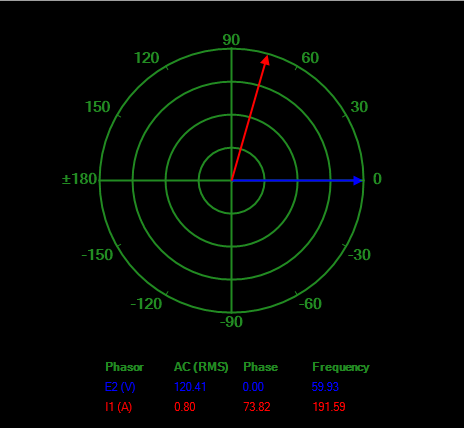
\includegraphics[width=0.75\textwidth]{figures/phasor-171.png}
	\end{center}
	\caption{}\label{fig1:}
\end{figure}

\begin{figure}[H]
	\begin{center}
		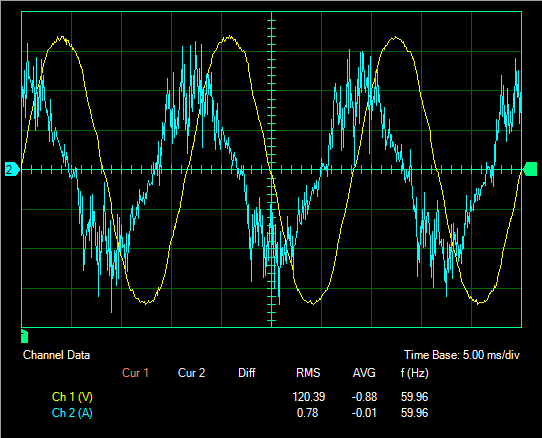
\includegraphics[width=0.75\textwidth]{figures/oscope-171.png}
	\end{center}
	\caption{}\label{fig2:}
\end{figure}

\begin{figure}[H]
	\begin{center}
		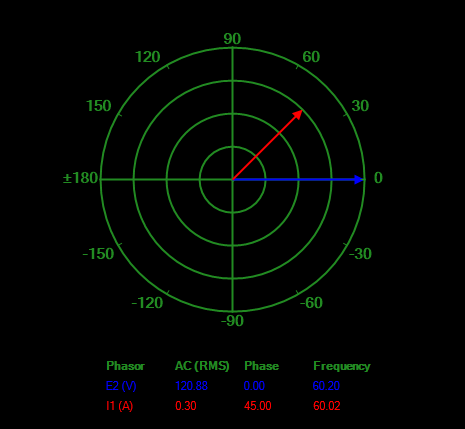
\includegraphics[width=0.75\textwidth]{figures/phasor-600.png}
	\end{center}
	\caption{}\label{fig3:}
\end{figure}

\begin{figure}[H]
	\begin{center}
		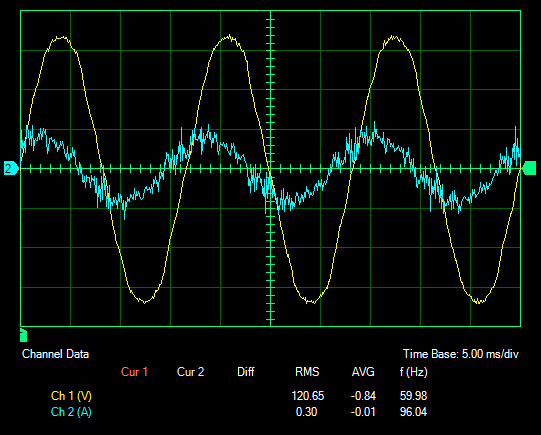
\includegraphics[width=0.75\textwidth]{figures/oscope-600.png}
	\end{center}
	\caption{}\label{fig4:}
\end{figure}

\begin{figure}[H]
	\begin{center}
		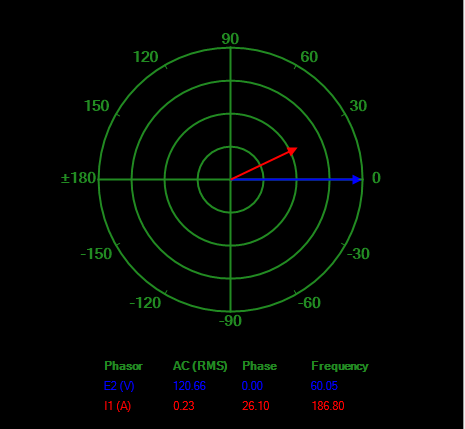
\includegraphics[width=0.75\textwidth]{figures/phasor-1200.png}
	\end{center}
	\caption{}\label{fig5:}
\end{figure}

\begin{figure}[H]
	\begin{center}
		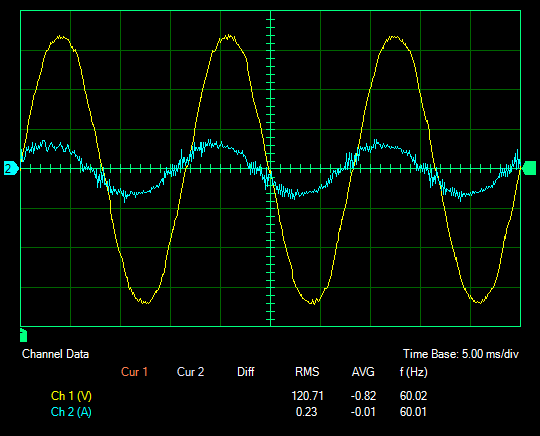
\includegraphics[width=0.75\textwidth]{figures/oscope-1200.png}
	\end{center}
	\caption{}\label{fig6:}
\end{figure}

\begin{figure}[H]
	\begin{center}
		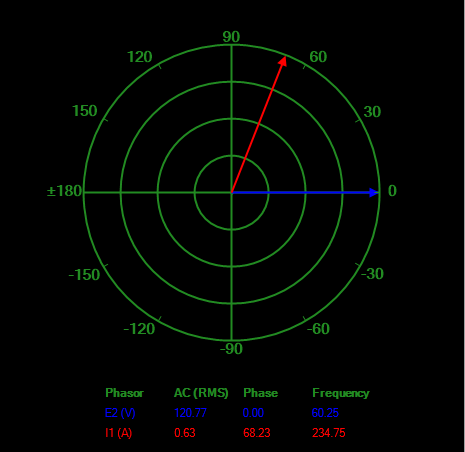
\includegraphics[width=0.75\textwidth]{figures/phasor-l-171.png}
	\end{center}
	\caption{}\label{fig7:}
\end{figure}

\begin{figure}[H]
	\begin{center}
		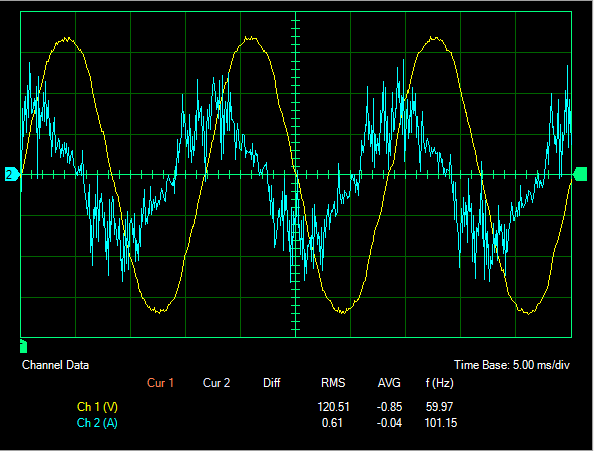
\includegraphics[width=0.75\textwidth]{figures/oscope-l-171.png}
	\end{center}
	\caption{}\label{fig8:}
\end{figure}

\begin{figure}[H]
	\begin{center}
		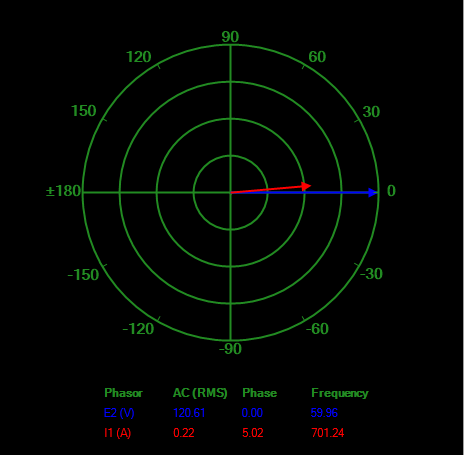
\includegraphics[width=0.75\textwidth]{figures/phasor-l-600.png}
	\end{center}
	\caption{}\label{fig9:}
\end{figure}

\begin{figure}[H]
	\begin{center}
		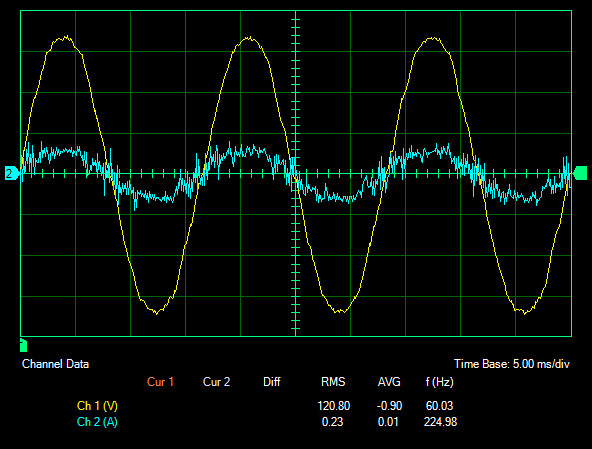
\includegraphics[width=0.75\textwidth]{figures/oscope-l-600.png}
	\end{center}
	\caption{}\label{fig10:}
\end{figure}

\begin{figure}[H]
	\begin{center}
		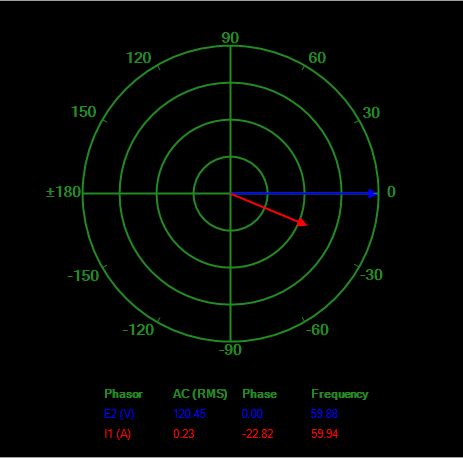
\includegraphics[width=0.75\textwidth]{figures/phasor-l-1200.png}
	\end{center}
	\caption{}\label{fig11:}
\end{figure}

\begin{figure}[H]
	\begin{center}
		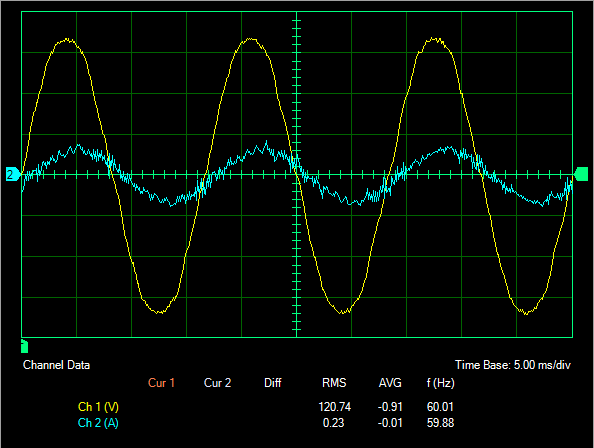
\includegraphics[width=0.75\textwidth]{figures/oscope-l-1200.png}
	\end{center}
	\caption{}\label{fig12:}
\end{figure}
